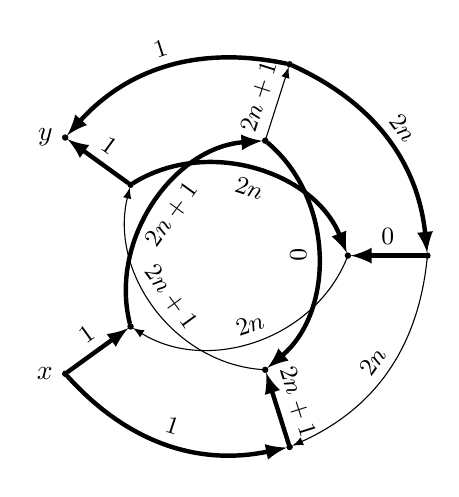
\begin{tikzpicture}[auto]
    
    \node (d0) [circle, draw, fill, scale=0.2, label=left:$x$] at (6, 12.93) {};
    \node (d1) [circle, draw, fill, scale=0.2, label=left:$y$] at (6, 15.93) {};
    \node (d2) [circle, draw, fill, scale=0.2] at (8.85, 16.86) {};
    \node (d3) [circle, draw, fill, scale=0.2] at (10.6, 14.43) {};
    \node (d4) [circle, draw, fill, scale=0.2] at (8.85, 12) {};
    \node (d5) [circle, draw, fill, scale=0.2] at (6.83, 13.53) {};
    \node (d6) [circle, draw, fill, scale=0.2] at (6.83, 15.33) {};
    \node (d7) [circle, draw, fill, scale=0.2] at (8.54, 15.89) {};
    \node (d8) [circle, draw, fill, scale=0.2] at (9.59, 14.43) {};
    \node (d9) [circle, draw, fill, scale=0.2] at (8.54, 12.98) {};

    \path[-latex]
    (d2) edge[ultra thick, bend right] node[sloped] {\small $1$} (d1)
    (d2) edge[ultra thick, bend left] node[sloped] {\small $2n$} (d3)
    (d3) edge[bend left] node[sloped] {\small $2n$} (d4)
    (d0) edge[ultra thick, bend right] node[sloped] {\small $1$} (d4)
    (d0) edge[ultra thick] node[sloped] {\small $1$} (d5)
    (d6) edge[ultra thick] node[sloped] {\small $1$} (d1)
    (d7) edge node[sloped] {\small $2n+1$} (d2)
    (d3) edge[ultra thick] node[sloped] {\small $0$} (d8)
    (d4) edge[ultra thick] node[sloped] {\small $2n+1$} (d9)
    (d5) edge[ultra thick, bend left=50] node[sloped, below] {\small $2n+1$} (d7)
    (d6) edge[ultra thick, bend left=50] node[sloped, below] {\small $2n$} (d8)
    (d7) edge[ultra thick, bend left=50] node[sloped, below] {\small $0$} (d9)
    (d8) edge[bend left=50] node[sloped, above] {\small $2n$} (d5)
    (d9) edge[bend left=50] node[sloped, above] {\small $2n+1$} (d6);
\end{tikzpicture}
